% This file provides an example Beamer presentation using the RWTH theme
% showcasing some of the more common options, similar to the Powerpoint version
% 12.11.2014: Revision 1 (Harold Bruintjes, Tim Lange)

% For RWTH, beamer should be loaded with class option t (top)
\documentclass[t]{beamer}

% Use fontspec to get Arial font
% Requires use of XeLaTeX
\usepackage{fontspec}
\setmainfont{Arial}
\setsansfont{Arial}
% Also force Arial for math for a more consistent look
\usepackage{unicode-math}

% https://tex.stackexchange.com/questions/426088/texlive-pretest-2018-beamer-and-subfig-collide
\makeatletter
\let\@@magyar@captionfix\relax
\makeatother

% German style date formatting (footer)
\usepackage[ddmmyyyy]{datetime}
\renewcommand{\dateseparator}{.}

\usepackage{MnSymbol,wasysym}

% Format the captions used for figures etc.
\usepackage[compatibility=false]{caption}
\captionsetup{singlelinecheck=off,justification=raggedleft,labelformat=empty,labelsep=none}

% PGFPlots is used for drawing some of the charts
\usepackage{pgfplots}
\pgfplotsset{compat=newest}
% This file contains some styles and macros for drawing charts similar to those of MS Office

\pgfplotsset{hor_barchart/.style={
  xbar=0mm,
  xmin=0,
  xtick=\empty,
  axis y line*=left,
  x axis line style={opacity=0},
  bar width=0.6cm,
  ytick=data,
  nodes near coords,
  every axis/.append style={font=\normalsize},
  every node near coord/.append style={font=\normalsize},
  nodes near coords align={horizontal},
  legend style={at={(0,-10mm)},anchor=north west,legend columns=-1,draw=none},
}}

\pgfplotsset{ver_barchart/.style={
  ybar=0mm,
  x = 4.5cm,
  ymin=0,
  ymajorgrids,
  axis x line*=bottom,
  y axis line style={opacity=0},
  bar width=0.8cm,
  enlarge x limits={0.15},
  xtick=data,
  nodes near coords,
  every axis/.append style={font=\normalsize},
  every node near coord/.append style={font=\normalsize},
  nodes near coords align={vertical},
  legend style={at={(0,-10mm)},anchor=north west,legend columns=-1,draw=none},
}}

\tikzstyle{chart}=[
    legend label/.style={font={\normalsize},anchor=west,align=left},
    legend box/.style={rectangle, draw=none, minimum size=5pt},
]

\tikzstyle{pie chart}=[
    chart,
    slice/.style={line cap=round, line join=round,draw=none},
    pie title/.style={font={\bf}},
    slice type/.style 2 args={
        ##1/.style={fill=##2},
        values of ##1/.style={}
    }
]

\newcommand{\pie}[3][]{
    \begin{scope}[#1]
    \pgfmathsetmacro{\curA}{90}
    \pgfmathsetmacro{\r}{1}
    \def\c{(0,0)}
    \node[pie title] at (90:1.3) {#2};
    \foreach \v/\s in{#3}{
        \pgfmathsetmacro{\deltaA}{\v/100*360}
        \pgfmathsetmacro{\nextA}{\curA + \deltaA}
        \pgfmathsetmacro{\midA}{(\curA+\nextA)/2}

        \path[slice,\s] \c
            -- +(\curA:\r)
            arc (\curA:\nextA:\r)
            -- cycle;

        %\begin{pgfonlayer}{foreground}
        % Position labels at 1.2 times radius (just outside of chart)
        \path \c -- node[pos=1.2,pie values,values of \s]{$\v\%$} +(\midA:\r);
        %\end{pgfonlayer}

        \global\let\curA\nextA
    }
    \end{scope}
}

% Custom legend (used for pie chart)
\newcommand{\legend}[2][]{
\begin{scope}[#1]
  \path
    \foreach \n/\s in {#2} {
      ++(0,-5pt) node[\s,legend box] {} +(5pt,0) node[legend label] {\n}
    };
\end{scope}
}


% Load the actual RWTH theme. Suggested is to load the full theme,
% as it requires some specific dimensions
\usetheme{rwth}

% -------------------- My Packages -------------------- %
\usepackage{hyperref}
\usepackage{xcolor}
\usepackage[utf8]{inputenc}
\usepackage{interval}
\usepackage[ngerman]{babel}
\usepackage{csquotes}
\usepackage{tikz}
\def\checkmark{\tikz\fill[scale=0.4](0,.35) -- (.25,0) -- (1,.7) -- (.25,.15) -- cycle;}

% \usepackage{fontspec}
\setmonofont{Roboto Mono}
\usepackage{minted}
\newcommand\pycode[1]{\inputminted[frame=lines, framesep=2mm, fontsize=\normalsize]{python}{#1}}

\definecolor{comment}{HTML}{aaaaaa} % italic
\definecolor{string}{HTML}{448c27}


%---------- Ich bin ein verdammter Künstler ----------
\usepackage{listings}
\definecolor{maroon}{RGB}{128, 0, 0}
\definecolor{pinegreen}{RGB}{1, 121, 111}
\definecolor{darkmidnightblue}{RGB}{0, 51, 102}
\definecolor{rwthblue}{RGB}{0, 84, 159}
% www.colorhexa.com for color references

% ---------- Hyperref -----------
\hypersetup{colorlinks=true,
            breaklinks=true,
            urlcolor=rwthblue,
            linkcolor=rwthblue,
            citecolor=rwthblue}
\def\UrlBreaks{\do\/\do-}
% -------------------------------


\begin{document}
\logo{
\includegraphics{logo.png}}

% Setup presentation information
\title{Back-Propagation and Algorithms for Training Artificial Neural Networks with TensorFlow}
\date{11. Dezember 2020}
\author{Gero Kauerauf}

\frame{\titlepage}

\section{Überblick}
% Frame with items
\begin{frame}
    \begin{itemize}
        \item Bildklassifizierung mit TensorFlow.Keras
        \begin{itemize}
            \item Was soll das Modell können?
            \item Der Datensatz
            \item Konstruktion des Python-Programms
        \end{itemize}
    \end{itemize}
\end{frame}

\section{Was soll unser Modell können?}
\begin{frame}
    \begin{itemize}
        \item Das Modell soll unterschiedliche Blumen erkennen können
        \item Der Datensatz besteht aus Blumenbildern, welche von Menschen kategorisiert wurden
        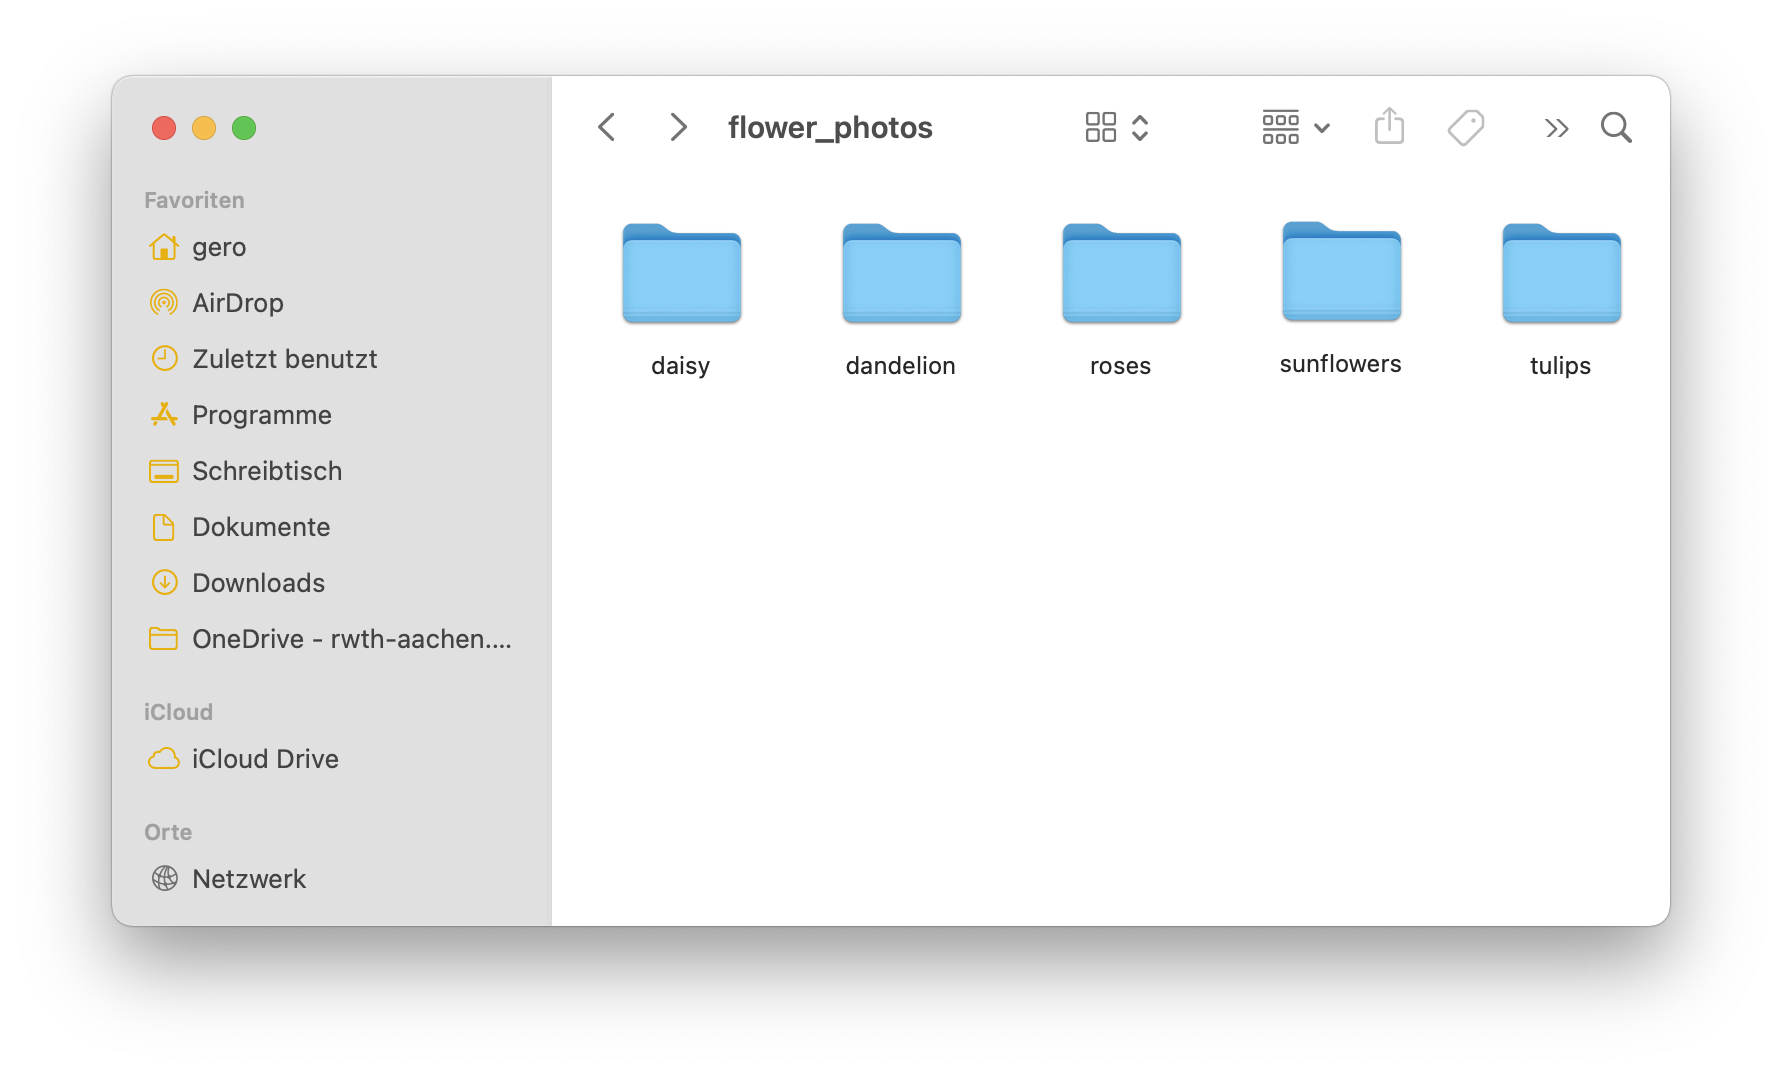
\includegraphics[width=0.5\textwidth]{teach-plots/flower-photos}
        \item Es gibt Bilder von Gänseblümchen, Löwenzahn, Rosen, Sonnenblumen und Tuplen
        \item Mit diesem Datensatz kann ein Modell trainiert werden, um Blumen unterscheiden zu können
    \end{itemize}
\end{frame}

\section{Datensatz}
\begin{frame}
    \begin{itemize}
        \item Beispielbilder.
    \end{itemize}
    \begin{figure}
        \centering
        \begin{minipage}{0.4\textwidth}
            \centering
            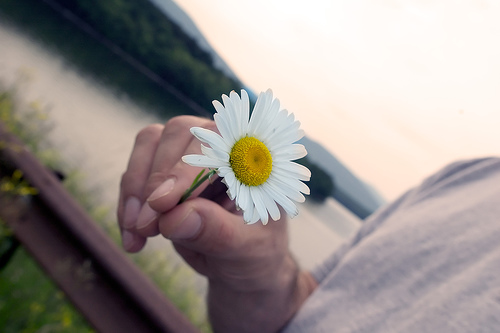
\includegraphics[width=0.8\textwidth]{./teach-plots/dandelion.jpg} % first figure itself
        \end{minipage}\hfill
        \begin{minipage}{0.4\textwidth}
            \centering
            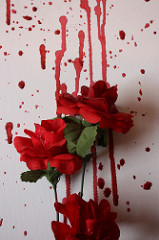
\includegraphics[width=0.5\textwidth]{./teach-plots/rose.jpg} % second figure itself
        \end{minipage}
    \end{figure}
    \begin{figure}
        \centering
        \begin{minipage}{0.4\textwidth}
            \centering
            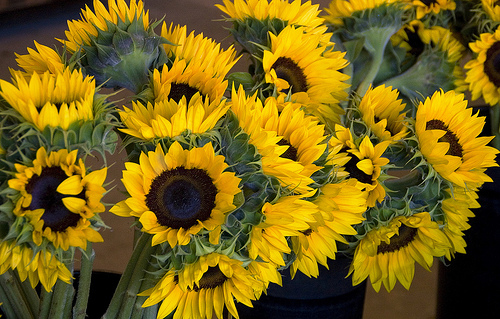
\includegraphics[width=0.8\textwidth]{./teach-plots/sunflower.jpg} % first figure itself
        \end{minipage}\hfill
        \begin{minipage}{0.4\textwidth}
            \centering
            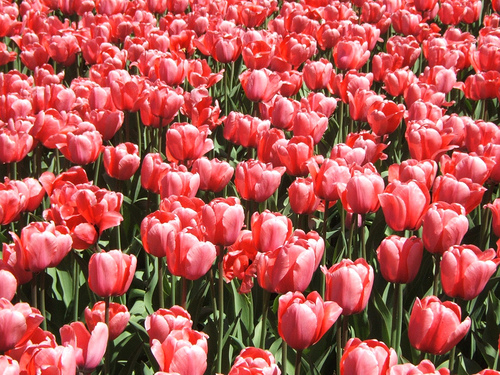
\includegraphics[width=0.68\textwidth]{./teach-plots/tulip.jpg} % second figure itself
        \end{minipage}
    \end{figure}
\end{frame}

\section{Datensatz}
\begin{frame}
    \begin{itemize}
        \item Zuerst laden wir den Datensatz
        \item Dazu definieren wir zuerst die Bildgrößen und die Batch-size
        \pycode{./code-snippets/dataset-params.py}
        \item Danach wird der Datensatz in einen Trainings- und einen Validierungssatz aufgeteilt
        \item Mit dem Trainingssatz wird dann das Modell trainiert
        \item Mit dem Validierungssatz wird das Modell nach dem Training beurteilt
    \end{itemize}
\end{frame}

\section{Datensatz}
\begin{frame}
    \begin{itemize}
        \item Dazu nutzen wir die Methode \texttt{image\_dataset\_from\_directory} aus \texttt{tf.keras.preprocessing}
        \pycode{./code-snippets/dataset-from-directory.py}
    \end{itemize}
\end{frame}

\section{Leistungsoptimierung}
\begin{frame}
    \begin{itemize}
        \item Wir verwenden zwei Methoden um die Performance beim Laden der Daten zu verbessern
        \item \texttt{Dataset.cache()}
        \begin{itemize}
            \item Geladene Bilder werden im RAM gelassen und nicht jedes mal erneut eingeladen
        \end{itemize}
        \item \texttt{Dataset.prefetch()}
        \begin{itemize}
            \item Datenvorverarbeitung und Modelltraining werden überlappt
            \item Im \(i\)-ten Trainingsschritt werden die Daten für den den \(i+1\)-ten Schritt gelesen.
        \end{itemize}
    \end{itemize}
\end{frame}

\section{Leistungsoptimierung}
\begin{frame}
    \begin{itemize}
        \item Ohne prefetching
    \end{itemize}
    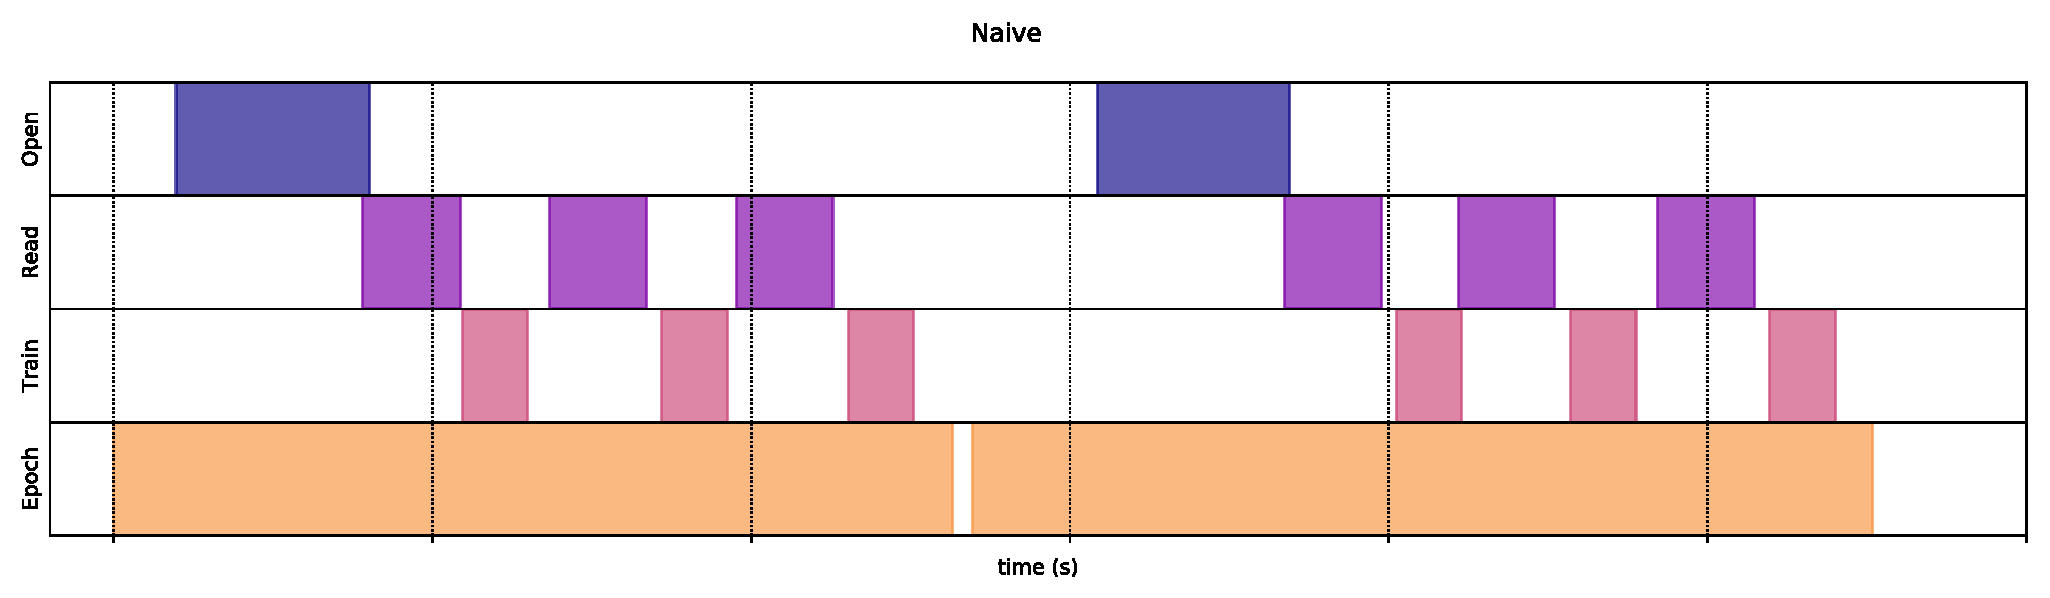
\includegraphics[width=0.7\textwidth]{teach-plots/naive-prefetching-crop.pdf}
    \begin{itemize}
        \item Mit prefetching
    \end{itemize}
    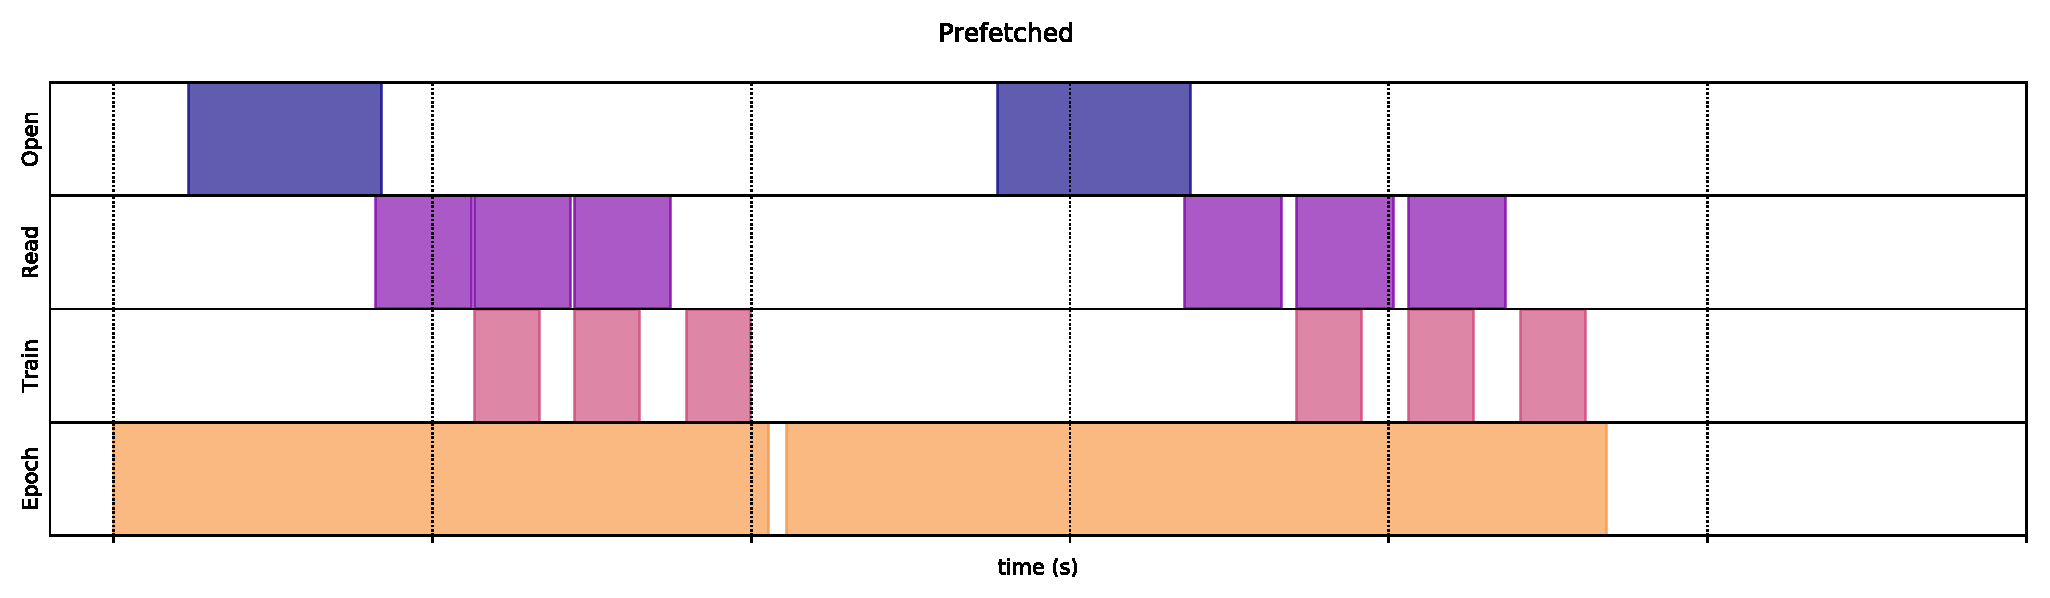
\includegraphics[width=0.7\textwidth]{teach-plots/prefetched-crop.pdf}
    \large\href{https://www.tensorflow.org/guide/data_performance}{https://www.tensorflow.org/guide/data\_performance}
\end{frame}

\section{Leistungsoptimierung}
\begin{frame}
    \begin{itemize}
        \item Wir nutzen die experimentelle Methode \texttt{AUTOTUNE}
        \item Diese passt die \texttt{buffer\_size} von \texttt{prefetch} dynamisch zur Laufzeit an
        \pycode{./code-snippets/dataset-optimize.py}
        \item Des weiteren ist es in der Praxis von Vorteil die Daten zu standardisieren
        \item Da der RGB-Farbraum das Interval \(\interval{0}{255}\) umfasst, können wir die Daten skalieren, indem wir mit einem Faktor von \(1./255\) multipilizieren
        \item Danach liegen die Werte jedes Pixels in \(\interval{0}{1}\)
        \newline  
        \item Es gibt nun zwei Möglichkeiten zu standardisieren
        \begin{itemize}
            \item Wir standardisieren den Datensatz
            \item Das erste Layer in unserem Modell skaliert die Eingabe \quad \textcolor{rwthblue}{\(\leftarrow\)} \textcolor{rwthblue}{\(\checkmark\)}
        \end{itemize}
    \end{itemize}
\end{frame}

\section{Sequentielles Modell}
\begin{frame}
    \begin{itemize}
        \item Als nächstes erstellen wir ein sequentielles Modell
        \item Dazu nutzen wir \texttt{tf.keras.Sequential}
        \pycode{./code-snippets/sequential-model-no-aug.py}
    \end{itemize}
\end{frame}

\section{Sequentielles Modell}
\begin{frame}
    \begin{itemize}
        \item Wir konfigurieren das Modell mit \texttt{tf.keras.Sequential.compile}
        \item Hierbei wählen wir den \emph{Optimierer}, die \emph{Fehlerfunktion} und die \emph{Metrik}
        \pycode{./code-snippets/model-compile.py}
        \item \texttt{adam} ist ein stochastisches Gradientenabstiegsverfahren, welches auf adaptiven Schätzungen der Momente ersten und zweiten Grades beruht
        \item \texttt{SparseCategoricalCrossentropy} ist eine Fehlerfunktion für mehrere Labels
        \item \texttt{accuracy} berechnet wie häufig die Klassifizierung durch das Modell mit der tatsächlichen Klasse übereinstimmt
    \end{itemize}
\end{frame}

\section{Training des Modells}
\begin{frame}
    \begin{itemize}
        \item Nachdem wir den Datensatz vorbereitet und das Modell konfiguriert haben, beginnt nun das Training
        \newline
        \item Wir trainieren das Modell 10 Epochen lang
        \item Das bedeutet wir iterieren im Training 10-mal über den Trainingsdatensatz
        \pycode{./code-snippets/model-fit.py}
    \end{itemize}
    \begin{itemize}
        \item Nun möchten wir natürlich sehen, wie gut das Training des Modells funktioniert hat
        \item Dazu zeichnen wir die Trainingsgeschichte mithilfe des Moduls \texttt{matplotlib}
    \end{itemize}
\end{frame}

% \section{Trainingsergebnisse}
% \begin{frame}
%     \begin{itemize}
%         \item Nun möchten wir natürlich sehen wie gut das Training des Modells funktioniert hat
%         \item Dazu zeichnen wir die Trainingsgeschichte mithilfe des Moduls \texttt{matplotlib}
%         \pycode{./code-snippets/plot-results.py}
%     \end{itemize}
% \end{frame}

\section{Trainingsergebnisse}
\begin{frame}
    \begin{itemize}
        \item Die gezeichnete Grafik enthält Informationen über den Verlauf des Trainings
    \end{itemize}
    \begin{figure}
        \begin{minipage}{0.5\textwidth}
            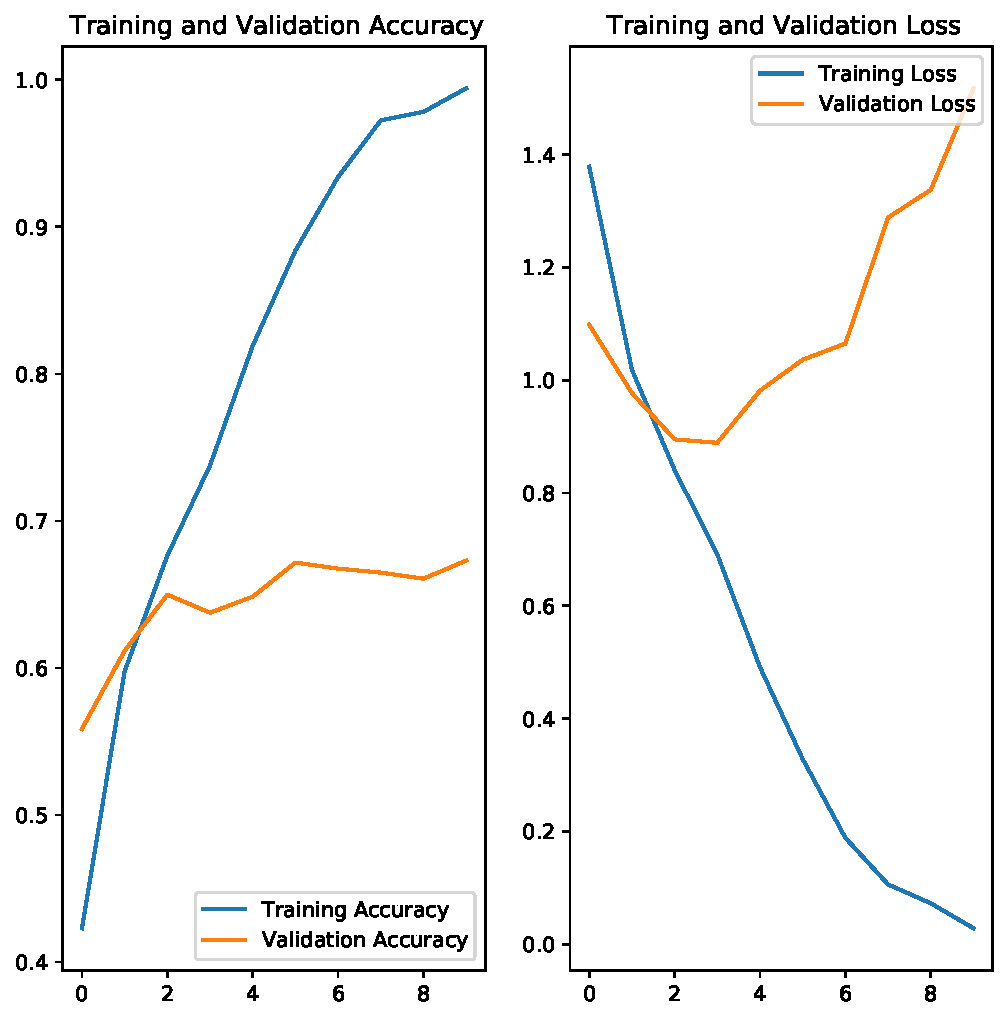
\includegraphics[width=\textwidth]{./teach-plots/pre_augmentation.pdf}
        \end{minipage}\hfill
        \begin{minipage}{0.5\textwidth}
            \begin{itemize}
                \item Die Genauigkeit der Vorhersagen \ldots
                \begin{itemize}
                    \item[\ldots] für den Trainingsdatensatz steigt
                    \item[\ldots] für den Validierungsdatensatz stagniert
                \end{itemize}
            \end{itemize}
        \end{minipage}
    \end{figure}
\end{frame}

\section{Overfitting}
\begin{frame}
    \begin{itemize}
        \item Der auftretende Effekt wird Overfitting (dt. Überanpassung) genannt
        \item Aufgrund des kleinen Umfangs unseres Datensatzes lernt das Modell den Trainingsdatensatz im Prinzip \enquote{auswendig}
        \item Es tritt also eine Überanpassung an den Trainingsdatensatz auf, das Modell lernt \enquote{ungewünschte} Details der Bilder
        \newline
        \item Wir können das Modell mit zwei Methoden verbessern
        \begin{itemize}
            \item[1.] Data augmentation (dt. Datenerweiterung)
            \item[2.] Dropout (dt. Rauswerfen)
        \end{itemize}
    \end{itemize}
\end{frame}

\section{Data augmentation}
\begin{frame}
    \begin{itemize}
        \item Um unseren Datensatz künstlich zu erweitern, können wir bereits im Datensatz enthaltene Bilder \enquote{leicht} verändern
        \item Dies ist zum Beispiel durch Spiegeln, Rotation oder Zoomen möglich
        \newline
        \item Dafür nutzen wir drei experimentelle Schichten aus TensorFlow
        \pycode{./code-snippets/data-aug.py}
    \end{itemize}
\end{frame}

\section{Verbessertes Modell}
\begin{frame}
    \begin{itemize}
        \item Zu unserem verbesserten Modell fügen wir nun noch eine \texttt{tf.keras.layers.Dropout}-Schicht hinzu
        \pycode{./code-snippets/improved-model.py}
    \end{itemize}
\end{frame}

\section{Training des verbesserten Modells}
\begin{frame}
    \begin{itemize}
        \item Nun kompilieren und trainieren wir das verbesserte Modell noch
        \pycode{./code-snippets/model-compile.py}
        \pycode{./code-snippets/improved-model-fit.py}
    \end{itemize}
\end{frame}

\section{Ergebnis der Verbesserung}
\begin{frame}
    \begin{figure}
        \begin{minipage}{0.5\textwidth}
            \begin{itemize}
                \item Vorher.
            \end{itemize}
            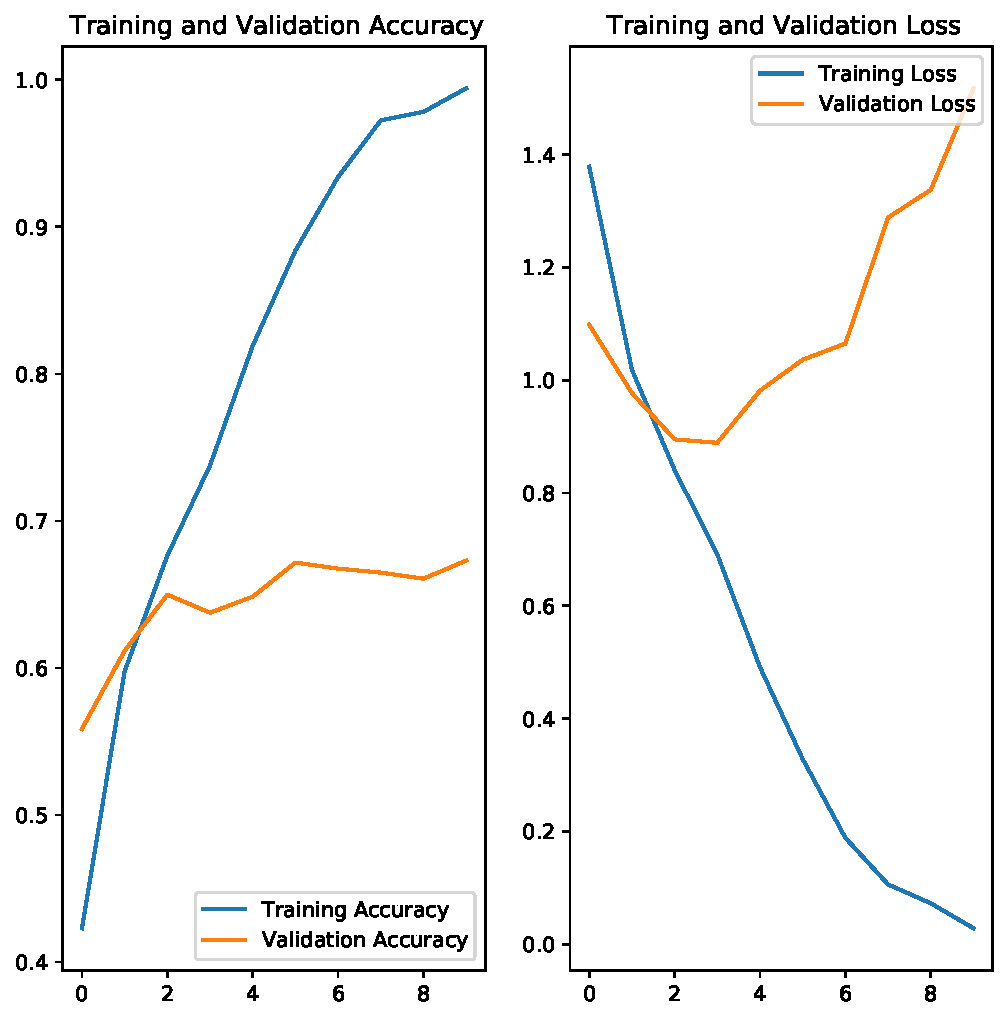
\includegraphics[width=\textwidth]{./teach-plots/pre_augmentation.pdf}
        \end{minipage}\hfill
        \begin{minipage}{0.5\textwidth}
            \begin{itemize}
                \item Nachher.
            \end{itemize}
            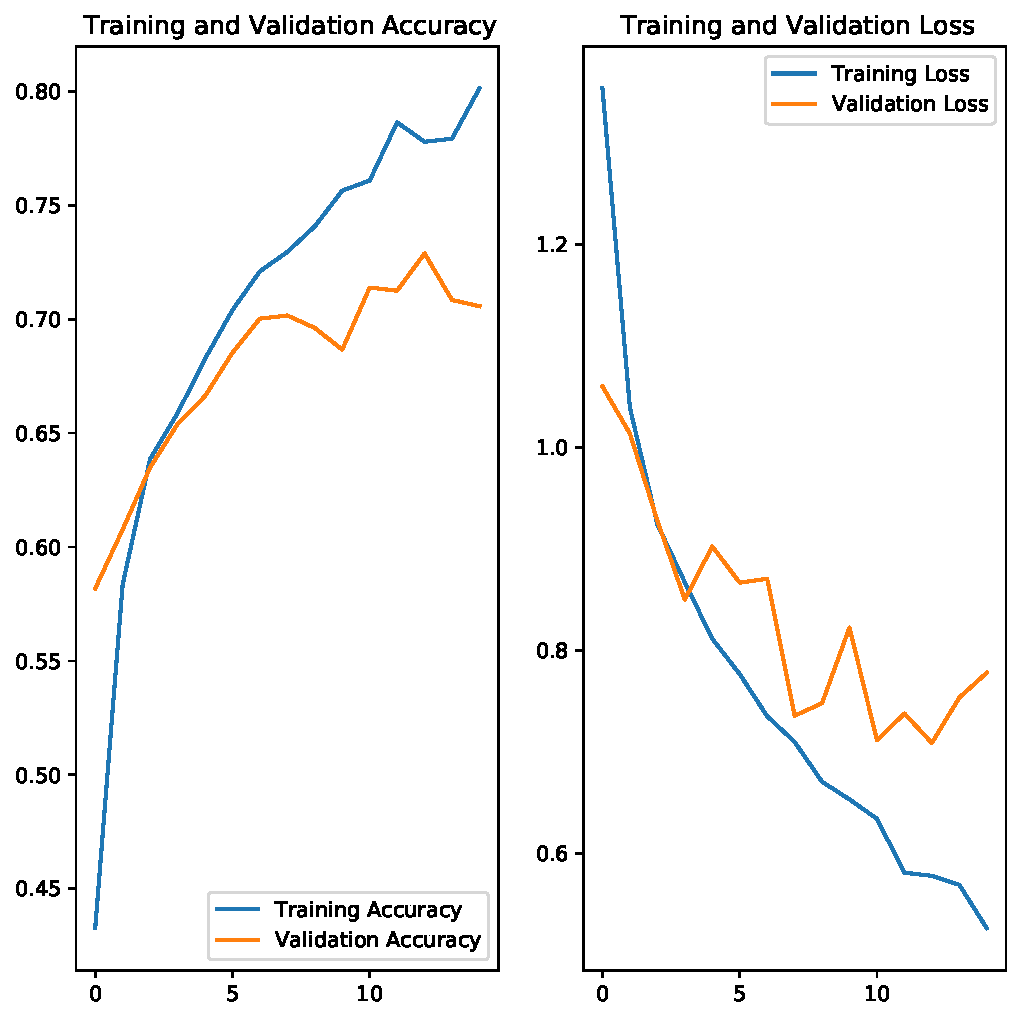
\includegraphics[width=\textwidth]{./teach-plots/post_augmentation.pdf}
        \end{minipage}
    \end{figure}
\end{frame}

\section{Vorhersagen von neuen Daten}
\begin{frame}
    \begin{itemize}
        \item Jetzt wollen wir natürlich auch Vorhersagen für beliebige (neue) Bilder machen
    \end{itemize}
    \pycode{./code-snippets/predict-new-image.py}
    \begin{minipage}{0.5\textwidth}
        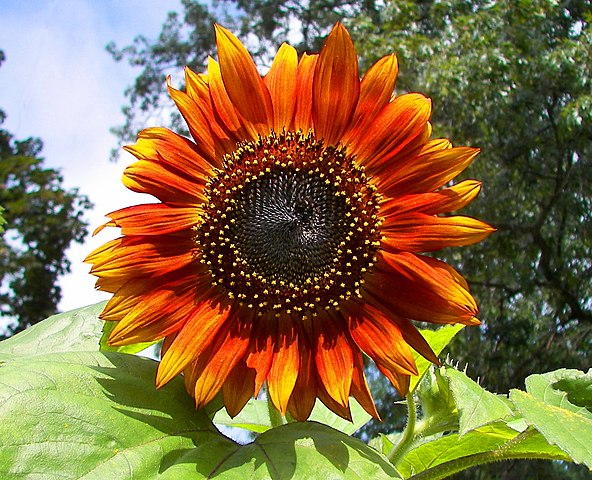
\includegraphics[width=0.75\textwidth]{./teach-plots/592px-Red_sunflower.jpg}
    \end{minipage}\hfill
    \begin{minipage}{0.5\textwidth}
        \begin{itemize}
            \item \textcolor{rwthblue}{Live Demonstration.}
        \end{itemize}
    \end{minipage}
\end{frame}

\section{Fazit}
\begin{frame}
    \begin{itemize}
        \item TensorFlow ist ein \emph{mächtiges} Modul für \textbf{Machine Learning}
        \newline
        \item Quellen
        \begin{itemize}
            \item \href{https://www.tensorflow.org/tutorials/images/classification}{https://www.tensorflow.org/tutorials/images/classification}
            \item \href{https://www.tensorflow.org/api\_docs/python/tf}{https://www.tensorflow.org/api\_docs/python/tf}
            \item \href{https://arxiv.org/pdf/1511.07122.pdf}{https://arxiv.org/pdf/1511.07122.pdf}
        \end{itemize}
    \end{itemize}
\end{frame}

\end{document}
